\documentclass{article}
\usepackage[utf8]{inputenc}
\usepackage[UKenglish]{babel}
%\renewcommand{\familydefault}{\sfdefault}
\usepackage{ifpdf}
\usepackage{hyperref}
\usepackage{graphicx}
\usepackage{caption}
\title{Ceph Mon: a technical overview}
\author{Paolo VIOTTI}
\date{\today}
\ifpdf
\hypersetup{
    pdfauthor={Paolo VIOTTI},
    pdftitle={Ceph Mon: a technical overview},
}
\fi
\begin{document}

\maketitle

\begin{abstract}
Ceph is a free software storage platform designed to provide object, block and file storage 
using computer clusters running on commodity hardware. 
Ceph's main design goals include high scalability, fault tolerance and low maintenance requirements.
This document provides an in-depth technical overview of the design of Ceph Monitor, 
i.e. the Ceph component in charge of maintaining a map of the cluster along with authorization information.
\end{abstract}

\section{Ceph: an introduction}
Ceph \cite{ceph} is a free software storage platform that provides object, block and file storage 
using computer clusters running on commodity hardware. 
Since its origin as a research project around 2006, 
Ceph has undergone constant and substantial development,
thus gaining popularity which is reflected by an ever increasing adoption as storage backend in state-of-the-art
high-end computing systems \cite{ceph-openstack}.

As illustrated in Fig. \ref{fig:stack}, Ceph exposes to application clients multiple APIs: 
\begin{itemize}
	\item a POSIX-compatible distributed file system (\textbf{Ceph FS}), built as Linux kernel module or user-space FUSE client;
	\item a REST-based storage gateway (\textbf{RADOSGW}) compatible with OpenStack Swift and Amazon S3;
	\item a block storage device (\textbf{RDB}) suitable for virtualization platforms making use of kernel 
	virtualization technologies such as QEMU or KVM.
\end{itemize}

\begin{center}
	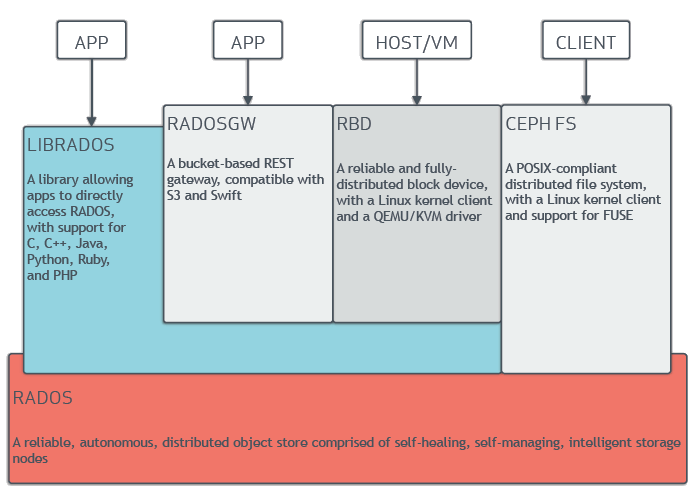
\includegraphics[scale=0.35]{figs/ceph-stack.png}
	\captionof{figure}{Ceph application stack}
	\label{fig:stack}
\end{center}

Beside, an application developer may even hook into the low level API exposed through \textbf{librados} 
and offered in several programming languages in order to directly connect with \textbf{RADOS} 
(\textit{Reliable Autonomic Distributed Object Store}), i.e. the inner object storage layer
that acts as foundation of the interfaces mentioned above.

The Ceph cluster consists of different components, running as distributed daemons:
\begin{itemize}
	\item Cluster monitors (\textit{ceph-mon}, or Mon) that keep track of active and failed cluster nodes;
	\item Metadata servers (\textit{ceph-mds}) that store the metadata of inodes and directories;
    \item Object storage devices (\textit{ceph-osd}) that actually store data on local filesystems;
    \item RESTful gateways (\textit{ceph-rgw}) that expose the object storage layer as an interface 
    compatible with Amazon S3 or OpenStack Swift APIs.
\end{itemize}

\section{Ceph Mon}

During runtime operations, Ceph OSD Daemons check up on other Ceph OSD Daemons and report their findings to the Ceph Monitor. You do not have to provide any settings.


\subsection{Architecture}

\begin{center}
	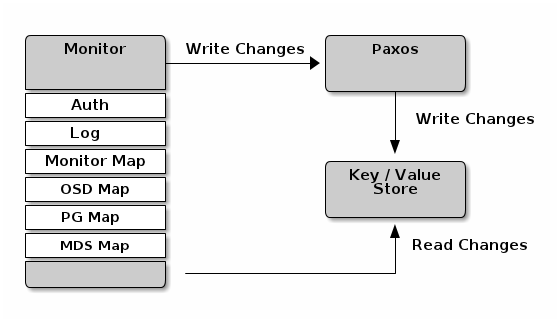
\includegraphics[scale=0.50]{figs/ceph-mon-arch.png}
	\captionof{figure}{Ceph Monitor high-level architecture}
	\label{fig:monarch}
\end{center}



\subsection{Code}


\subsection{Additional notes}


\begin{thebibliography}{1}

  \bibitem{ceph} Ceph storage platform. \url{http://ceph.com/} 

  \bibitem{ceph-openstack} OpenStack User Survey Insights: November 2014. \\
  \url{http://perma.cc/367D-G5YN} 

  %\bibitem{fo} Bob Tadashi Wakabayashi {\em Anti-Foreignism and Western
  %Learning in Early-Modern Japan} 1986: Harvard University Press.

\end{thebibliography}
	
\end{document}
